%************************************************
\chapter{Newton's Ring}
%************************************************
\begin{flushright}
August 14 and 21, 2012
\end{flushright}
\section{Aim}
	To study the fringes of equal thickness in the Newton's ring setup and hence determine the wave-length of sodium light.
\section{Apparatus}
	Sodium vapour lamp, travelling microscope, lens assembly consisting of a plane glass plate and a planoconvex lens, spherometer, magnifying glass, vernier callipers and a tiltable  glass plate assembly.

\section{Theory}
	Light when shone on a plano-convex lens in contact with a flat glass plate, produces circular successive dark and bright interference fringes, called Newton's rings. The radius of these fringes depends on both the wavelength and the radius of curvature of the lens. The objective of the experiment is to determine the wavelength of light, by experimentally determining the radius of curvature and analysing the fringes.\\
	To derive the basic relationship, let's first consider the geometry of the problem (refer to \autoref{1_fig1}). For a spherical lens of radius of curvature $R$, consider a circle at a distance $d$ from the bottom plane, with radius $r$. Invoking Pythagoras Theorem, we have
	\begin{equation}
		d=R- (R^{2} - r^{2})^{1/2}
	\end{equation}
	Now let's consider a thin film problem (refer to \autoref{1_fig2}). Optical path distance can be evaluated as $n_{2}(AB + BC) - n_{1}(AD)$. Also, from geometry, we have $AB=BC=\frac{d}{\cos{\theta _{2}}}$. Plus, $AD=2d(\tan{\theta_{2}}\sin{\theta_{1}})$. Therefore from Snell's Law, we can further simplify the optical path difference to $2n_{2}d(\frac{1-\sin^{2}{\theta_{2}}}{\cos{\theta_{2}}})$ which can be rewritten as:
	\begin{equation}	
		2n_{2}d\cos{\theta_{2}}=m\lambda
	\end{equation}
	for constructive interference. \\

	For newton's ring, we can approximate $\cos{\theta_{2}}$ to be $1$. Thus we have $2nt=(m+\frac{1}{2})\lambda$ where $n=1$ for air. We therefore get
	\begin{equation}
		2nt=(m+\frac{1}{2})\lambda
	\end{equation}
	for the bright interference, m=0,1, etc. \\
	We also have $r_{m}=(R\lambda m)^{1/2}$ from which we obtain directly a linear  relation
	\begin{equation}
		(D_{m})^{2}=4R\lambda m
	\end{equation}
	Further, we can use the difference to evaluation $\lambda$ as follows:
	\begin{equation}
		\frac{(D_{m+n})^{2} - (D_{m})^{2}}{4Rn}=\lambda
	\end{equation}

\section{Observations and Calculations}
	$h$ was found out to be 0.25 mm = 0.025 cm. \\
	$l$ was found out to be $\frac{4.668+3.874}{2}=4.271$ cm. (For details, refer to \autoref{1_l}) \\
	Using these, $R=\frac{l^{2}}{6h} + \frac{h}{2}$ turns out to be $121.6211$ cm.\\
	 \\
	Observations for diameter of the ring are given in \autoref{1_Diameter}.\\
	Slope of the graph of Diameter Squared, $D_{m}^{2}$ vs Order of Ring, $m$ was found to be $0.0291$ cm. (\autoref{1_graph})\\
	Using the relation
	\begin{equation}
		(D_{m})^{2}=4R\lambda m
	\end{equation}
	$\lambda=598.16\pm 3.25\%$ nm (where the error is calculated from the standard deviation of the slope).
	\begin{table}
		\myfloatalign
		\begin{tabularx}{\textwidth}{Xlll}
			\hline
			\tableheadline{Order of Dark Ring $m$} 	&	\tableheadline{Left (cm)} & \tableheadline{Right (cm)}\\
			\hline
				6	&	5.800	&	6.260\\
				9	&	5.755	&	6.304\\
				12	&	5.720	&	6.350\\
				13	&	5.704	&	6.360\\
				14	&	5.700	&	6.370\\
				15	&	5.670	&	6.382\\
				16	&	5.665	&	6.400\\
				19	&	5.650	&	6.420\\
				23	&	5.605	&	6.459\\
				25	&	5.600	&	6.467\\
			\hline
		\end{tabularx}
		\caption{Diameter of Newton's Ring}
		\label{1_Diameter}
	\end{table}

	\begin{table}
		\myfloatalign
		\begin{tabularx}{\textwidth}{Xlll}
			\hline
			\tableheadline{Main Scale (cm)}	& \tableheadline{Vernier Scale Division} & \tableheadline{Reading (cm)}\\
			\hline
			\tableheadline{Outer $l$}\\
				4.6	& 34 & 4.668\\
				4.6	& 35 & 4.670\\
				4.6	& 34 & 4.668\\	
			\hline
			\tableheadline{Inner $l$}\\
				3.8	& 37 & 3.874\\
				3.8	& 38 & 3.876\\
				3.8	& 37 & 3.874\\		
			\hline
		\end{tabularx}
		\caption{Measurement of $l$ of spherometer}
		\label{1_l}
	\end{table}

	\begin{figure}[bth]
		\begin{center}
			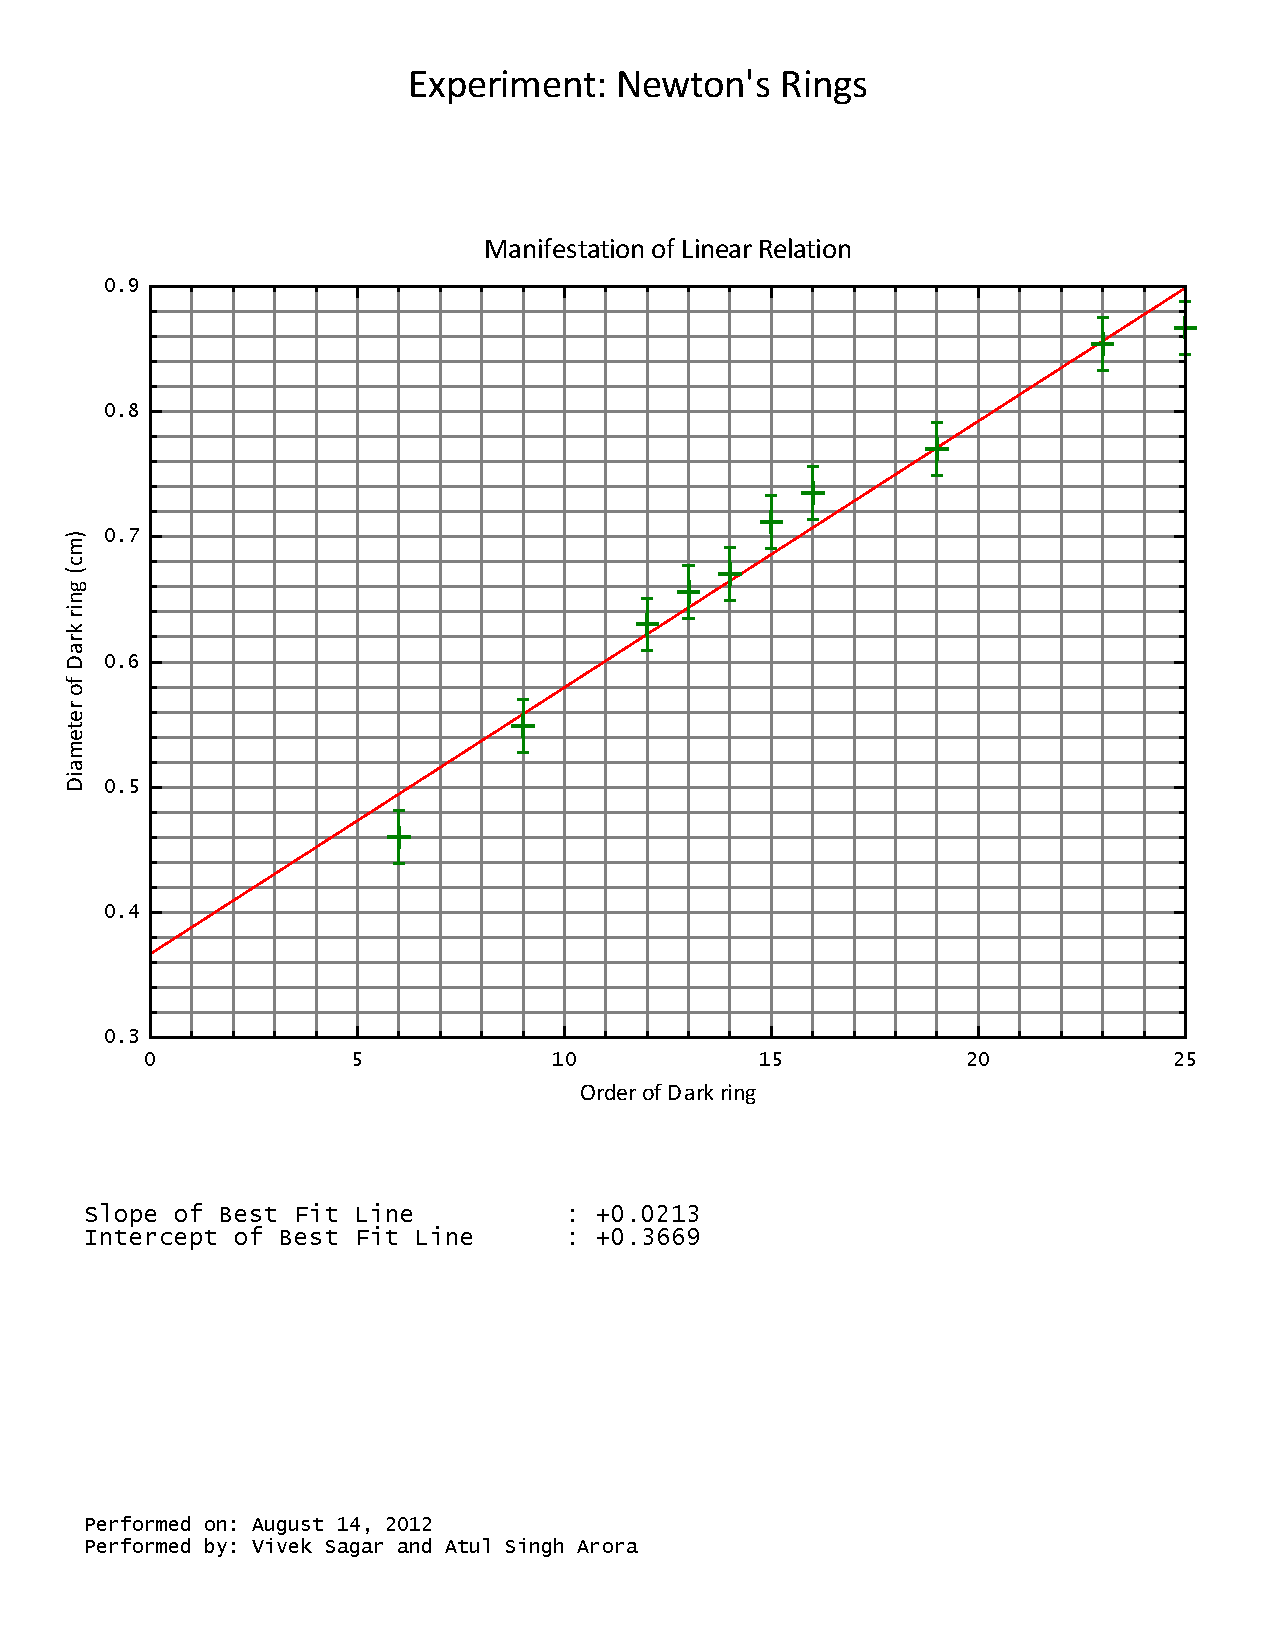
\includegraphics[width=1.3\linewidth]{gfx/1_linear.pdf}
		\end{center}
	\caption[Diameter Squared vs Order of Ring]{Least Square Fit of Diameter Squared vs Order of Ring}
	\label{1_graph}
	\end{figure}

	\begin{figure}[bth]
		\begin{center}
			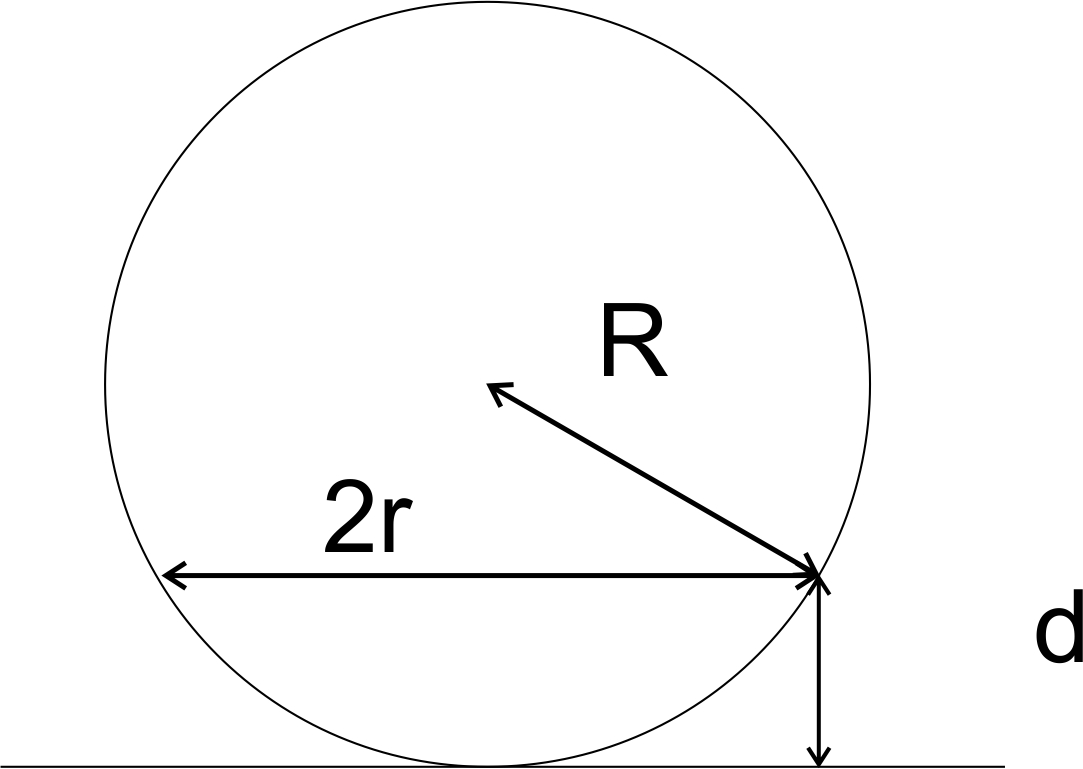
\includegraphics[width=0.8\linewidth]{gfx/E1_A.jpg}
		\end{center}
	\caption[Spherical Lens]{Spherical Lens}
	\label{1_fig1}
	\end{figure}

	\begin{figure}[bth]
		\begin{center}
			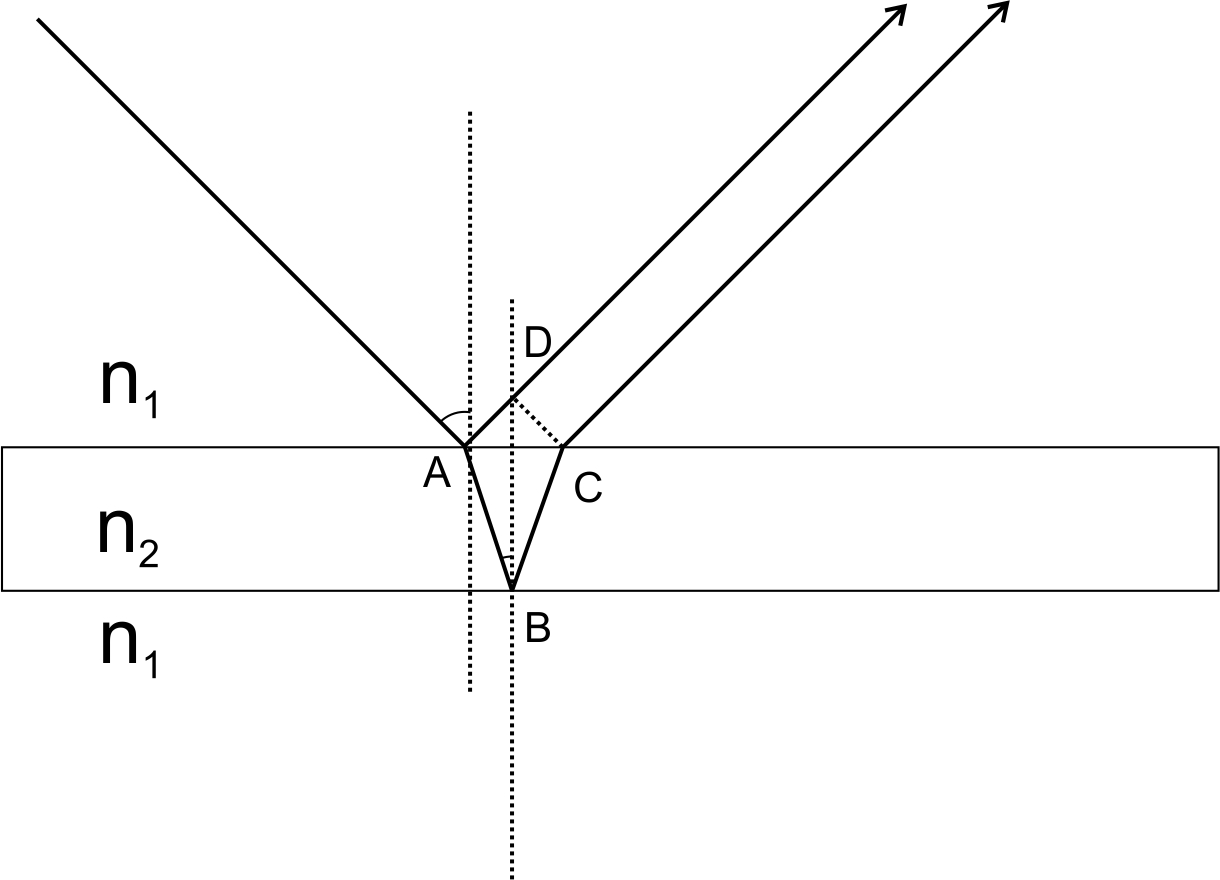
\includegraphics[width=0.8\linewidth]{gfx/E1_B.jpg}
		\end{center}
	\caption[Thin Film Interference]{Thin Film Interference}
	\label{1_fig2}
	\end{figure}

\section{Result}
	The expected wavelength of sodium vapour lamp is $589.5$ nm. \\
	Experimentally, the wavelength, $\lambda$ was found to be \\
	$598.16\pm 3.25\%$ nm (standard deviation of the slope).\\
	Accuracy error is $1.5\%$, within the precision.
